code
Latex
download
content_copy
expand_less
\documentclass{article}
\usepackage{amsmath}
\usepackage{amssymb}
\usepackage{graphicx}
\usepackage{tikz}
\usepackage{pgfplots}
\pgfplotsset{compat=1.18}
\usepackage{booktabs}
\usepackage{xcolor}

\newenvironment{lesson-meta}{}{}
\newenvironment{item-analysis}{}{}
\newenvironment{model-discuss}{}{}
\newenvironment{concept-box}{}{}
\newenvironment{concept-summary}{}{}
\newenvironment{example}[1]{\textbf{Example #1}}{}
\newenvironment{tryit}[1]{\textbf{Try It! #1}}{}
\newenvironment{practice}[2]{\textbf{#1} (DOK #2)}{}
\newenvironment{te-addendum}[2]{\textbf{TE (#1 - #2)}}{}
\newcommand{\answer}[1]{\textbf{Answer:} #1}
\newcommand{\placeholder}[2]{[\textit{Placeholder: #1 - #2}]}
\newcommand{\uncertain}[2]{#1}
\newcommand{\te}[1]{\textit{#1}}

\begin{document}

\begin{lesson-meta}
\textbf{LESSON 4-3: Multiplying and Dividing Rational Expressions}

\textbf{Objective}
Students will be able to:
\begin{itemize}
    \item Use the structure of rational expressions to rewrite simple rational expressions in different forms.
    \item Understand that rational expressions form a system analogous to the system of rational numbers and use that understanding to multiply and divide rational expressions.
\end{itemize}

\textbf{Essential Understanding}
Rational expressions form a system similar to the system of rational numbers and can be multiplied and divided by applying the properties of operations as they apply to rational expressions.

\textbf{Vocabulary Builder}
\begin{itemize}
    \item \textbf{Review Vocabulary:} greatest common factor, rational number, rational expression
    \item \textbf{New Vocabulary:} simplified form of a rational expression
\end{itemize}

\textbf{Vocabulary Activity}
Review the terms \textit{rational number} and \textit{rational expression} with students. Relate the two by discussing how the terms \textit{greatest common factor} and \textit{simplified form} would apply to both rational numbers and rational expressions. Have students match the rational number and rational expression with its simplified form.
\begin{itemize}
    \item $\frac{4}{8} \longrightarrow \frac{1}{2}$
    \item $\frac{(x+4)(x-2)}{(x-3)(x-2)} \longrightarrow \frac{x+4}{x-3}$
\end{itemize}
\end{lesson-meta}

\begin{item-analysis}
\begin{tabular}{ccc}
\toprule
\textbf{Example} & \textbf{Items} & \textbf{DOK} \\
\midrule
1 & 20, 21, 38 & 1 \\
1 & 11, 14--16, 19 & 2 \\
2 & 22--25, 39 & 1 \\
2 & 17, 38 & 2 \\
3 & 26, 27 & 1 \\
3 & 12, 18 & 2 \\
4 & 28, 29 & 1 \\
5 & 30--33 & 1 \\
5 & 40 & 2 \\
5 & 13 & 3 \\
6 & 34, 35 & 1 \\
6 & 36, 37 & 2 \\
\bottomrule
\end{tabular}
\end{item-analysis}

\begin{te-addendum}{Explore \& Reason}{Implement Tasks that Promote Reasoning and Problem Solving}
Q: What do you notice about the graph of the function?
\answer{[Sample: $x$-intercept = $-2$; $y$-intercept = $2$; The function is linear.]}
\end{te-addendum}

\begin{te-addendum}{Explore \& Reason}{Support Productive Struggle in Learning Mathematics}
Q: Why is it important to know the domain of a function?
\answer{[The domain needs to make sense for the scenario. For example, a real-world problem involving time should remain in Quadrant I on a graph because all numbers should be positive. Also, some values of $x$ cause the function to be undefined, so they cannot be included in the domain.]}

\textbf{For Early Finishers}
Q: Sketch the function $y = -x + 4$. What is the domain of the function?
\answer{[all real numbers]}
Q: Sketch the graph of the function, excluding $-4$ from the domain. Describe the new graph created.
\answer{[The graph is a linear function with a negative slope and an opening at $x = -4$. The $x$-intercept is 4, and the $y$-intercept is 4.]}
\end{te-addendum}

\begin{model-discuss}
\textbf{EXPLORE \& REASON}

Consider the following graph of the function $y = x + 2$.

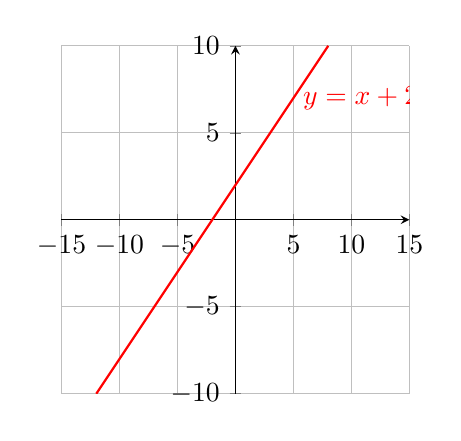
\begin{tikzpicture}
\begin{axis}[
    width=6cm, height=6cm,
    axis lines=middle,
    xmin=-15, xmax=15,
    ymin=-10, ymax=10,
    xtick={-15,-10,-5,5,10,15},
    ytick={-10,-5,5,10},
    grid=both
]
\addplot[domain=-12:8, color=red, thick] {x+2};
\node[right, red] at (5,7) {$y = x + 2$};
\end{axis}
\end{tikzpicture}

\textbf{A.} What is the domain of this function?
\answer{all real numbers.}

\textbf{B.} Sketch a function that resembles the graph, but restrict its domain to exclude 2.
\answer{
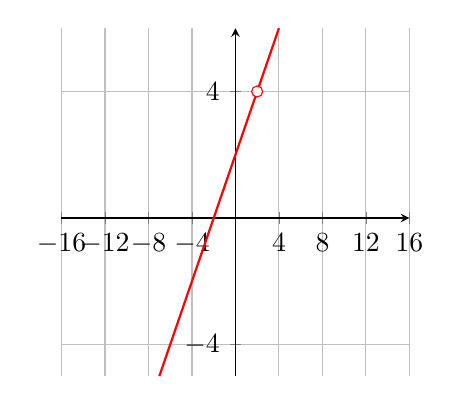
\begin{tikzpicture}
\begin{axis}[
    width=6cm, height=6cm,
    axis lines=middle,
    xmin=-16, xmax=16,
    ymin=-5, ymax=6,
    xtick={-16,-12,-8,-4,4,8,12,16},
    ytick={-4,4},
    grid=both
]
\addplot[domain=-7:4, color=red, thick] {x+2};
\addplot[color=red, fill=white, mark=*] coordinates {(2,4)};
\end{axis}
\end{tikzpicture}
}

\textbf{C. Use Structure} Consider the function you have sketched. What kind of function might have a graph like this? Explain.
\answer{An equation where the denominator equals zero when $x = 2$. For example, $y = \frac{2x - 4}{x - 2}$.}
\end{model-discuss}

\begin{te-addendum}{Explore \& Reason}{Facilitate Meaningful Mathematical Discourse}
Discuss the difference between functions that have asymptotes and functions that have discontinuities.
Q: How does the exclusion of an $x$-value in a function's domain due to an asymptote compare to the exclusion of an $x$-value in a function's domain at a single point?
\answer{[An asymptote occurs when there is an expression in a fraction's denominator that equals zero and the numerator is not equal to zero for that value. The graph curves on either side of the asymptote and gets close to but never touches it. When the exclusion is at a single point, the graph appears to have a "hole" at the excluded value, with the function attaining values "close" to the hole.]}
\end{te-addendum}

\begin{concept-box}
\textbf{HABITS OF MIND} \\
\textbf{Reason} Does the graph of $y = \frac{2x+6}{x+3}$ have a vertical asymptote at $x = -3$? Explain. \\
\answer{[No; because the function approaches the point $(-3, 2)$ from both sides, there is a hole at $x = -3$ instead of an asymptote.]}
\end{concept-box}

\begin{concept-box}
\textbf{ESSENTIAL QUESTION} \\
How does multiplying and dividing fractions help you multiply and divide rational expressions?
\end{concept-box}

\begin{te-addendum}{1}{Establish Mathematics Goals to Focus Learning}
Introduce students to rational expressions. Explain that multiplying and dividing rational expressions is similar to multiplying and dividing rational numbers.
\end{te-addendum}

\begin{example}{1}
\textbf{Write Equivalent Rational Expressions}

Write an expression that is equivalent to $\frac{x+4}{x-9}$. For what domain are the expressions equivalent?

You can multiply by factors of 1 in any form to write equivalent rational expressions. In this Example, multiply by $\frac{x-6}{x-6}$ and $\frac{x}{x}$.

$\frac{x+4}{x-9} \cdot \frac{x-6}{x-6} \cdot \frac{x}{x}$
$= \frac{(x+4)(x-6)x}{(x-9)(x-6)x}$
$= \frac{x^3 - 2x^2 - 24x}{x^3 - 15x^2 + 54x}$

Since the denominator $x^3 - 15x^2 + 54x = x(x-9)(x-6)$ the expression is undefined for $0, -9$, and $6$. So the domain must exclude $0, -9$, and $6$.

Expressions are equivalent for all values of $x$ that are in both domains. Therefore, $\frac{x+4}{x-9}$ is equivalent to $\frac{x^3 - 2x^2 - 24x}{x^3 - 15x^2 + 54x}$ over the domain $\{x \mid \text{all real numbers where } x \neq 0, 6, \text{ or } -9\}$.
\end{example}

\begin{te-addendum}{1}{Use and Connect Mathematical Representations}
Q: Why is the domain for the identity different from the domain of just the original rational expression?
\answer{[Because the equivalence of two expressions must occur where the expressions are both defined.]}
Q: Why does the denominator affect the domain but the numerator does not?
\answer{[For real values of $x$, a rational expression is the quotient of real numbers. Quotients of real numbers are undefined only when the denominator is 0, and does not depend on the numerator.]}
Q: How else can you write an expression equivalent to the original rational expression?
\answer{[Multiplying $\frac{x+3}{x+9}$ by any other rational expression, such as $\frac{x}{x}$, $\frac{2-x}{2-x}$, $x^2$, etc., will result in an equivalent rational expression to the original.]}
\end{te-addendum}

\begin{tryit}{1}
Write an expression equivalent to $\frac{x-4}{x}$ over the domain $\{x \mid x \neq 0 \text{ or } -2\}$. \\
\answer{$\frac{x^2 - 2x - 8}{x^2 + 2x}$}
\end{tryit}

\begin{te-addendum}{1}{Elicit and Use Evidence of Student Thinking}
Q: What are the common factors that occur in both the numerator and the denominator?
\answer{[$x+2$]}
\end{te-addendum}

\begin{te-addendum}{1}{Common Error}
Students may think that a common factor $(x - 2)$ results in excluding $-2$ from the domain. Have students find the expression or factor when $x = 2$. Then ask them for another factor that could result in excluding $-2$ from the domain.
\end{te-addendum}

\begin{example}{2}
\textbf{Simplify a Rational Expression}

What is the simplified form of the rational expression? What is the domain for which the identity between the two expressions is valid?

$\frac{4 - x^2}{x^2 + 3x - 10}$

The \textbf{simplified form of a rational expression} has no common factors, other than 1, in the numerator and the denominator.

Factor each polynomial in the numerator and denominator. The domain is all real numbers except $2$ and $-5$.
$\frac{4 - x^2}{x^2 + 3x - 10} = \frac{(2 - x)(2 + x)}{(x - 2)(x + 5)}$

Common factors divide to 1.
$= \frac{-1(x - 2)(x + 2)}{(x - 2)(x + 5)} = -1 \cdot \frac{x + 2}{x + 5} = -\frac{x + 2}{x + 5}$

The simplified form of $\frac{4 - x^2}{x^2 + 3x - 10}$ is $-\frac{x + 2}{x + 5}$ for $x \neq 2$ or $-5$.
\end{example}

\begin{te-addendum}{2}{Pose Purposeful Questions}
Q: Why is $-1$ factored out of $2 - x$ in the numerator?
\answer{[If you factor out $-1$, you can divide out the common factor $x - 2$.]}
Q: Why can you cross out factors that divide to 1?
\answer{[A rational expression with factors that divide to 1 can be written as 1 times another rational expression, and 1 is not typically written in products.]}
\end{te-addendum}

\begin{tryit}{2}
Simplify each expression and state the domain. \\
\textbf{a.} $\frac{x^2 + 2x + 1}{x^3 - 2x^2 - 3x}$ \qquad \textbf{b.} $\frac{x^3 + 4x^2 - x - 4}{x^2 + 3x - 4}$ \\
\answer{\textbf{a.} $\frac{x+1}{x(x-3)}$ for all $x$ except $0, -1, \text{ and } 3$ \qquad \textbf{b.} $x + 1$ for all $x$ except $1 \text{ and } -4$}
\end{tryit}

\begin{example}{3}
\textbf{Multiply Rational Expressions}

\textbf{A.} What is the product of $\frac{2xy}{z}$ and $\frac{3x^2}{4yz}$?

To multiply rational expressions, follow a similar method to that for multiplying two numerical fractions.
$\frac{2xy}{z} \cdot \frac{3x^2}{4yz} = \frac{(2xy)(3x^2)}{z(4yz)} = \frac{2 \cdot 3 \cdot x \cdot x^2 \cdot y}{2 \cdot 2 \cdot y \cdot z \cdot z}$
Identify common factors that divide to 1.
$= \frac{3x^3}{2z^2}$

The product is $\frac{3x^3}{2z^2}$ for $y \neq 0$ and $z \neq 0$.

\textbf{B.} What is the product of $\frac{5x}{x+3} \cdot \frac{x^2 + x - 6}{x^2 + 2x + 1} \cdot \frac{x^2 + x}{5x - 10}$ in simplified form?

$\frac{5x}{x+3} \cdot \frac{x^2 + x - 6}{x^2 + 2x + 1} \cdot \frac{x^2 + x}{5x - 10} = \frac{5x}{x+3} \cdot \frac{(x-2)(x+3)}{(x+1)(x+1)} \cdot \frac{x(x+1)}{5(x-2)}$
$= \frac{5x(x-2)(x+3)x(x+1)}{5(x+3)(x+1)(x+1)(x-2)}$
$= \frac{x^2}{x+1}$

So $\frac{5x}{x+3} \cdot \frac{x^2 + x - 6}{x^2 + 2x + 1} \cdot \frac{x^2 + x}{5x - 10} = \frac{x^2}{x+1}$ for $x \neq -3, -1, \text{ or } 2$.
\end{example}

\begin{te-addendum}{3}{Pose Purposeful Questions}
\textbf{PART A} \\
Q: How can you determine that the domain is $z \neq 0$ and $y \neq 0$ by looking at the rational expressions?
\answer{[The denominator cannot equal 0 because the rational expression would be undefined. Therefore, $z \neq 0$ and $y \neq 0$ because multiplying 0 by any number is 0.]}

\textbf{PART B} \\
Q: Why do you factor the expressions in the numerator and the denominator?
\answer{[You can divide out the common factors, and you can determine the restrictions on the domain by using the Zero Product Property.]}
\end{te-addendum}

\begin{tryit}{3}
Find the simplified form of each product, and state the domain. \\
\textbf{a.} $\frac{x^2 - 16}{9 - x} \cdot \frac{x^2 + x - 90}{x^2 + 14x + 40}$ \qquad \textbf{b.} $\frac{x+3}{4x} \cdot \frac{3x - 18}{6x + 18} \cdot \frac{x^2}{4x + 12}$ \\
\answer{\textbf{a.} $-(x - 4)$ for all $x$ except $9, -10, \text{ and } -4$ \qquad \textbf{b.} $\frac{x(x-6)}{32(x+3)}$ for all $x$ except $0 \text{ and } -3$}
\end{tryit}

\begin{concept-box}
\textbf{HABITS OF MIND} \\
\textbf{Critique Reasoning} Bailey simplified the rational expression $\frac{x^2 + 2x + 4}{x^2 + x + 2}$ by dividing out the $x^2$-terms and then dividing out a factor of $x+2$ to get 2 as the simplified form of the rational expression. Is Bailey correct? Why or why not? \\
\answer{[No; you cannot eliminate terms from the numerator and denominator if they are bound by addition. You must factor the expression first, and then eliminate like factors.]}
\end{concept-box}

\begin{te-addendum}{3}{RtISupport}
\textbf{Extend Student Thinking} \\
Challenge students to write an expression as the product of two rational expressions with the given domain. \\
Q: The domain of the product of two rational expressions is all real numbers except $0, -3$, and $6$.
\answer{[Sample: $\frac{1}{x^2 + 3x} \cdot \frac{1}{x - 6}$]}
\end{te-addendum}

\begin{example}{4}
\textbf{Multiply a Rational Expression by a Polynomial}

What is the product of $\frac{x+2}{x^2 - 16}$ and $x^3 + 4x^2 - 12x$?

$\frac{x+2}{x^2 - 16} \cdot (x^3 + 4x^2 - 12x) = \frac{x+2}{x^2 - 16} \cdot \frac{x^3 + 4x^2 - 12x}{1}$

Write 1 in the denominator to keep track of positions of factors.
$= \frac{(x+2)x(x^2 + 4x - 12)}{1(x^2 - 16)}$
$= \frac{x(x+2)(x+6)(x-2)}{(x+4)(x-4)}$

The domain is $x \neq -4, \text{ or } 4$.

So $\frac{x+2}{x^2 - 16} \cdot (x^3 + 4x^2 - 12x) = \frac{x(x+2)(x+6)(x-2)}{x^2 - 16}$ for $x \neq -4 \text{ or } 4$.
\end{example}

\begin{te-addendum}{4}{Use and Connect Mathematical Representations}
Q: What do you already know about multiplying a fraction and a whole number that is helpful here?
\answer{[To multiply a fraction and a whole number, you need to also make the whole number a fraction with a denominator of 1.]}
Q: Is there a number for $x$ that would make $x^2 + 4 = 0$?
\answer{[No; squaring any number, whether negative or positive, results in a positive number. Adding two positive numbers will never equal 0.]}
\end{te-addendum}

\begin{tryit}{4}
Find the simplified form of each product and the domain. \\
\textbf{a.} $\frac{x^2 - 4}{6x^2 - 13x - 5} \cdot (2x^3 - 3x^2 - 5x)$ \qquad \textbf{b.} $\frac{3x^2 + 6x}{x^2 - 49} \cdot (x^2 + 9x + 14)$ \\
\answer{\textbf{a.} $\frac{x^2(x+2)(x-2)(x+1)}{3x+1}$ for all $x$ except $\frac{5}{2} \text{ and } -\frac{1}{3}$ \qquad \textbf{b.} $\frac{3x(x+2)^2}{x-7}$ for all $x$ except $7 \text{ and } -7$}
\end{tryit}

\begin{concept-box}
\textbf{HABITS OF MIND} \\
\textbf{Generalize} Why is it important to identify the domain of a rational expression before you simplify it rather than after? \\
\answer{[Simplifying the expression may eliminate some values where the original expression is undefined.]}
\end{concept-box}

\begin{example}{5}
\textbf{Divide Rational Expressions}

What is the quotient of $\frac{x^3 + 3x^2 + 3x + 1}{1 - x^2}$ and $\frac{x^2 + 5x + 4}{x^2 + 3x - 4}$?

Multiply by the reciprocal of the divisor.
$\frac{x^3 + 3x^2 + 3x + 1}{1 - x^2} \div \frac{x^2 + 5x + 4}{x^2 + 3x - 4} = \frac{x^3 + 3x^2 + 3x + 1}{1 - x^2} \cdot \frac{x^2 + 3x - 4}{x^2 + 5x + 4}$
$= \frac{(x+1)(x+1)(x+1)}{-1(x-1)(x+1)} \cdot \frac{(x+4)(x-1)}{(x+4)(x+1)}$
$= -(x+1)$

The domain is $x \neq -4, -1, \text{ or } 1$.

The quotient is $-(x+1)$, $x \neq -4, -1, \text{ or } 1$.
\end{example}

\begin{te-addendum}{5}{Pose Purposeful Questions}
Q: Why do you factor out $-1$?
\answer{[The factoring out of $-1$ allows you to divide common factors from the numerator and the denominator.]}
Q: How is dividing rational expressions similar to dividing fractions?
\answer{[You multiply by the reciprocal of the divisor.]}
\end{te-addendum}

\begin{te-addendum}{5}{RtISupport}
\textbf{Support Struggling Students} \\
Students have the opportunity for guided practice in dividing two rational expressions. \\
Divide $\frac{3x^3 + 6x^2 + 3x}{x+2} \div \frac{x^2+x}{x+2}$. \\
Multiply by the reciprocal of the divisor. Factor the numerators and denominators individually. Divide out the common factors. \\
Q: How do you decide what can be factored out of each expression? \answer{[Find the greatest common factor.]} \\
Q: What are the quotient and the domain? \answer{[$3(x+1); x \neq -2, -1, 0$]}
\end{te-addendum}

\begin{tryit}{5}
Find the simplified quotient and the domain of each expression. \\
\textbf{a.} $\frac{1}{x^2 + 9x} \div \frac{6 - x}{3x^2 - 18x}$ \qquad \textbf{b.} $\frac{2x^2 - 12x}{x + 5} \div \frac{x - 6}{x + 5}$ \\
\answer{\textbf{a.} $-\frac{3}{x+9}$ for all $x$ except $0, -9, \text{ and } 6$ \qquad \textbf{b.} $2x$ for all $x$ except $6 \text{ and } -5$}
\end{tryit}

\begin{example}{6}
\textbf{Use Division of Rational Expressions}

A company is evaluating two packaging options for its product line. The more efficient design will have the lesser ratio of surface area to volume. Should the company use packages that are cylinders or rectangular prisms?

\textbf{Option 1:} A rectangular prism with a square base (sides $2x$, height $2x$)
Surface Area: $2(2x)^2 + 4(2x)^2 = 8x^2 + 16x^2 = 24x^2$
Volume: $(2x)^3 = 8x^3$

\textbf{Option 2:} A cylinder with the same height as the prism, and diameter equal to the side length of the prism's base (diameter $2x$, height $2x$)
Surface Area: $2\pi x^2 + 2\pi x(2x) = 2\pi x^2 + 4\pi x^2 = 6\pi x^2$
Volume: $\pi x^2(2x) = 2\pi x^3$

The efficiency ratio is $\frac{SA}{V}$, where SA represents surface area and V represents volume.

\textbf{Option 1:}
$\frac{SA}{V} = \frac{24x^2}{8x^3} = \frac{3}{x}$

\textbf{Option 2:}
$\frac{SA}{V} = \frac{6\pi x^2}{2\pi x^3} = \frac{3}{x}$

The company can now compare the efficiency ratio of the package designs.
Prism: $\frac{3}{x}$ \qquad Cylinder: $\frac{3}{x}$

In this example, the efficiency ratio of the cylinder is equal to that of the prism. So the company should choose their package design based on other criteria. Regardless of what positive value is selected for $x$, the efficiency ratios for these two package designs will be the same.
\end{example}

\begin{te-addendum}{6}{Pose Purposeful Questions}
Q: What does it mean to have \textit{the lesser ratio of surface area to volume}?
\answer{[the division of surface area by volume that results in a smaller rational expression]}
Q: How do the efficiency ratios of the rectangular prism and the cylinder compare to each other?
\answer{[The rectangular prisms and the cylinder will always have the same efficiency ratio, regardless of the $x$-value selected.]}
\end{te-addendum}

\begin{te-addendum}{6}{ELLAddendum}
\textbf{SPEAKING BEGINNING}
When you evaluate something, you assign it a value or level of importance. Display a pen, a stapler, a paper clip, and a cell phone. Have students discuss the following questions in small groups.
Q: How you would arrange these items from lowest to highest in value?
\answer{[paper clip, pen, stapler, cell phone]}
Q: Why would the packaging with a lesser ratio of surface area to volume be more valuable to a company?
\answer{[If the company spends less on packaging, they can make a larger profit.]}

\textbf{READING DEVELOPING}
Have students read the problem statement in the example. Have students point to the words \textit{ratio, surface area,} and \textit{volume} as they read them.
Q: What does \textit{surface area} mean?
\answer{[the sum of the areas of all of the outside surfaces of an object]}
Q: What does \textit{volume} mean?
\answer{[the capacity an object can hold, or the amount of space it takes up]}
Q: Why is the design with the lesser ratio of surface area to volume more efficient?
\answer{[because the packaging would use less material to contain a given volume]}

\textbf{LISTENING EXPANDING}
Distribute a piece of construction paper and a pair of scissors to pairs of students. Ask students to cut the paper into 5 or 6 polygons and mix them up. Have one person put the puzzle pieces back together while the other records the time it takes. Then switch roles. Have students repeat this exercise with their eyes closed. Listen to the definition of \textit{efficient}: "performing in the best possible manner with the least waste of time and effort."
Q: Which method of putting the puzzle together was more efficient? Explain.
\answer{[The first method was more efficient.]}
\end{te-addendum}

\begin{tryit}{6}
The company compares the ratios of surface area to volume for two more containers. One is a rectangular prism with a square base. The other is a rectangular prism with a rectangular base. One side of the base is equal to the side length of the first container, and the other side is twice as long. The surface area of this second container is $4x^2 + 6xh$. The heights of the two containers are equal. Which has the smaller surface area-to-volume ratio? \\
\answer{The efficiency ratio for the prism with the rectangular base is less than that for the prism with the square base.}
\end{tryit}

\begin{concept-box}
\textbf{HABITS OF MIND} \\
\textbf{Use Structure} Is the domain of the quotient $\frac{2x^2 - 12x}{x+5} \div \left(\frac{x - 6}{x+5}\right)$ different from the domain of the product $\left(\frac{2x^2 - 12x}{x+5}\right)\left(\frac{x+5}{x-6}\right)$? Explain. \\
\answer{[Yes; the domain of the product includes the value $x = 6$, while the domain of the quotient does not include $x = 6$.]}
\end{concept-box}

\begin{concept-summary}
\textbf{Products and Quotients of Rational Expressions}

\begin{tabular}{lp{4cm}p{4cm}p{4cm}}
\toprule
& \textbf{Multiply} & \textbf{Multiply an Integer or a Polynomial} & \textbf{Divide} \\
\midrule
\textbf{RATIONAL} &
$\frac{3x}{x+1} \cdot \frac{x^2+x}{3x-6}$ \newline The domain is $x \neq -1 \text{ or } 2$. &
$\frac{x+2}{x^2-4} \cdot (x^2-2x) = \frac{x+2}{x^2-4} \cdot \frac{x^2-2x}{1}$ \newline The domain is $x \neq -2 \text{ or } 2$. &
$\frac{1-x^2}{x^2+3x-4} \div \frac{x+1}{x+4} = \frac{1-x^2}{x^2+3x-4} \cdot \frac{x+4}{x+1}$ \newline The domain is $x \neq -4, -1, \text{ or } 1$. \\
\midrule
\textbf{WORDS} &
Identify common factors and simplify. &
Write the polynomial as a rational expression with 1 in the denominator. Then multiply. &
Multiply by the reciprocal of the divisor. \\
\bottomrule
\end{tabular}

\textbf{Do You UNDERSTAND?}
\begin{enumerate}
    \item \textbf{ESSENTIAL QUESTION} How does multiplying and dividing fractions help you multiply and divide rational expressions?
    \item \textbf{Vocabulary} In your own words, define rational expression and provide an example of a rational expression.
    \item \textbf{Error Analysis} A student divided the rational expressions as follows:
    $\frac{4x}{5y} \div \frac{20x^2}{25y^2} = \frac{4x}{5y} \cdot \frac{4x}{5y} = \frac{16x^2}{25y^2}$. Describe and correct the errors the student made.
    \item \textbf{Communicate Precisely} Why do you have to state the domain when simplifying rational expressions?
\end{enumerate}

\textbf{Do You KNOW HOW?}
\begin{enumerate}
\setcounter{enumi}{4}
    \item What is the simplified form of the rational expression $\frac{x^2-36}{x^2+3x-18}$? What is the domain?
\end{enumerate}
Find the simplified form of each product, and state the domain.
\begin{enumerate}
\setcounter{enumi}{5}
    \item $\frac{4x^2y^2}{3z} \cdot \frac{15z^2}{20xy^3}$
    \item $\frac{y+3}{y+2} \cdot \frac{y^2+4y+4}{y^2-9}$
    \item $\frac{x^2+3x-10}{x^2-25} \cdot (x^2-9x+20)$
\end{enumerate}
Find the simplified form of each quotient, and state the domain.
\begin{enumerate}
\setcounter{enumi}{8}
    \item $\frac{x^3+14x^2+49x}{x^2+3x-28} \div (x+7)$
    \item $\frac{6x^3+21x^2-12x}{x^3+x^2-36x-36} \div \frac{12x^2-6x}{4x^2-144}$
\end{enumerate}

\textbf{Answers:}
\begin{enumerate}
    \item The steps and operations used to multiply and divide rational expressions are similar to those used with fractions.
    \item A rational expression is the ratio of two polynomials that has a domain of all real numbers except those for which the denominator equals zero; Sample: $\frac{3x^2 + 6x}{9x}$
    \item The student was supposed to multiply by the reciprocal. The student also did not place any restrictions on the domain. The rational expression should be $\frac{y}{x}, x \neq 0, y \neq 0$.
    \item When the denominator equals 0, fractions are undefined.
    \item $\frac{x-6}{x-3}$ for all $x$ except $-6$ and $3$
    \item $\frac{xz}{y}, x \neq 0, y \neq 0, \text{ and } z \neq 0$
    \item $\frac{y+2}{y-3}, y \neq -3, 3, \text{ or } -2$
    \item $(x-2)(x - 4)$ for all $x$ except $5$ and $-5$
    \item $\frac{x}{x-4}$ for all $x$ except $4$ and $-7$
    \item $\frac{2x(x+4)}{(x+1)}$ for all $x$ except $-6, 6, -1, 0, \text{ and } \frac{1}{2}$
\end{enumerate}
\end{concept-summary}

\begin{te-addendum}{Exercise 9}{Common Error}
Students may struggle with division when the divisor is a polynomial instead of a rational expression. Ask students how the polynomial can be written as a rational expression. Then ask students how they can write the quotient of rational expressions as a product of rational expressions.
\end{te-addendum}

\textbf{PRACTICE \& PROBLEM SOLVING}

\begin{practice}{11}{2}
\textbf{Reason} Explain why $\frac{4x^2 - 7}{4x^2 - 7} = 1$ is a valid identity under the domain of all real numbers except $\pm \frac{\sqrt{7}}{2}$. \\
\answer{Using the difference of two squares formula, $\frac{4x^2 - 7}{4x^2 - 7} = \frac{(2x + \sqrt{7})(2x - \sqrt{7})}{(2x + \sqrt{7})(2x - \sqrt{7})}$. Both factors on the numerator and denominator divide to 1, so $\frac{4x^2 - 7}{4x^2 - 7} = 1$ over all elements of the domain, which is all real numbers except $\pm \frac{\sqrt{7}}{2}$.}
\end{practice}

\begin{practice}{12}{2}
\textbf{Error Analysis} Describe the error a student made in multiplying and simplifying
$\frac{x+2}{x-2} \cdot \frac{x^2 - 4}{x^2 + x - 2} = \frac{x+2}{x-2} \cdot \frac{(x+2)(x-2)}{(x+2)(x-1)} = \frac{x+2}{x-1} \rightarrow \frac{2}{-1}$ \\
\answer{The student cannot cancel the $x$'s in $x+2$ and $x-1$ because only common factors, not terms, can be canceled.}
\end{practice}

\begin{practice}{13}{3}
\textbf{Higher Order Thinking} Why are rational expressions closed under multiplication and division? \\
\answer{Sample: $\frac{a}{b} \cdot \frac{c}{d} = \frac{ac}{bd}$, $\frac{a}{b} \div \frac{c}{d} = \frac{a}{b} \cdot \frac{d}{c} = \frac{ad}{bc}$}
\end{practice}

\begin{practice}{14}{2}
\textbf{Use Appropriate Tools} Explain why domain restrictions are necessary to show that the rational expressions $\frac{-6x^2 + 21x}{3x}$ and $-2x + 7$ are equivalent. What is true about the graphs at $x = 0$ and why? \\
\answer{Sample answer: Domain restrictions are needed because you may not be able to tell just from graphs when two expressions are not equivalent. The graphs of $y = \frac{-6x^2 + 21x}{3x}$ and $y = -2x + 7$ may look identical, but using the trace feature or a table values, $y = \frac{-6x^2 + 21x}{3x}$ is undefined at $x = 0$, while $y = -2x + 7$ is equal to 7 at $x = 0$.}
\end{practice}

\begin{practice}{15}{2}
\textbf{Generalize} Explain the similarities between rational numbers and rational expressions. \\
\answer{A rational number is the ratio of two integers, while a rational expression is a ratio of two polynomials.}
\end{practice}

\begin{practice}{16}{2}
\textbf{Use Structure} Determine whether $\frac{5x + 11}{6x + 11} = \frac{5}{6}$ is sometimes, always, or never true. Justify your reasoning. \\
\answer{Never; when you cross multiply, you get $30x + 66 = 30x + 55$; since $66 \neq 55$, there is no real number $x$ for which that equation is true.}
\end{practice}

\begin{practice}{17}{2}
\textbf{Construct Arguments} Explain how you can tell whether a rational expression is in simplest form. \\
\answer{A rational expression is in simplest form when the numerator and denominator have no common factors other than 1.}
\end{practice}

\begin{practice}{18}{2}
\textbf{Communicate Precisely} When multiplying $\frac{15}{x} \cdot \frac{x}{3} = 5$, is it necessary to make the restriction $x \neq 0$? Why or why not? \\
\answer{Yes; even though the factor of $x$ was canceled out, the original fractions cannot be undefined, so the restriction is necessary.}
\end{practice}

\begin{practice}{19}{2}
\textbf{Reason} If the denominator of a rational expression is $x^3 + 3x^2 - 10x$, what value(s) must be restricted from the domain for $x$? \\
\answer{$-5, 0, 2$}
\end{practice}

Write an equivalent expression over the given domain.
\begin{practice}{20}{1}
$\frac{x(x - 2)}{(x - 5)}$ for all $x$ except 5 and $-6$ \\
\answer{$\frac{x^3 + 4x^2 - 12x}{x^2 + x - 30}$}
\end{practice}

\begin{practice}{21}{1}
$\frac{3x}{x - 2}$ for all $x$ except 2 and $-5$ \\
\answer{$\frac{3x^2 + 15x}{x^2 + 3x - 10}$}
\end{practice}

What is the simplified form of each rational expression? What is the domain?
\begin{practice}{22}{1}
$\frac{y^2 - 5y - 24}{y^2 + 3y}$ \\
\answer{$\frac{y - 8}{y}$ for all $y$ except $0$ and $-3$}
\end{practice}

\begin{practice}{23}{1}
$\frac{ab^3 - 9ab}{12ab^2 + 12ab - 144a}$ \\
\answer{$\frac{b(b+3)}{12(b+4)}$ for all real numbers except $a = 0, b = -4 \text{ and } 3$}
\end{practice}

\begin{practice}{24}{1}
$\frac{x^2 + 8x + 15}{x^2 - x - 12}$ \\
\answer{$\frac{x+5}{x-4}, x \neq -3, 4$}
\end{practice}

\begin{practice}{25}{1}
$\frac{x^3 + 9x^2 - 10x}{x^3 - 9x^2 - 10x}$ \\
\answer{$\frac{(x+10)(x-1)}{(x-10)(x+1)}, x \neq -1, 0, 10$}
\end{practice}

Find the product and the domain.
\begin{practice}{26}{1}
$\frac{x^2 + 6x + 8}{x^2 + 4x + 3} \cdot \frac{x + 3}{x + 2}$ \\
\answer{$\frac{x+4}{x+1}$ for all $x$ except $-3, -2, \text{ and } -1$}
\end{practice}

\begin{practice}{27}{1}
$\frac{(x - y)^2}{x + y} \cdot \frac{3x + 3y}{x^2 - y^2}$ \\
\answer{$\frac{3(x-y)}{x+y}$ for all real numbers except $x = y \text{ or } x = -y$}
\end{practice}

\begin{practice}{28}{1}
$\frac{(x + 5)}{(x^3 - 25x)} \cdot (2x^3 - 11x^2 + 5x)$ \\
\answer{$\frac{2x-1}{x-5}$ for all $x$ except $0, -5, \text{ and } 5$}
\end{practice}

\begin{practice}{29}{1}
$\frac{(2x^2 - 10x)}{(x - 5)(x^2 - 1)} \cdot (3x^2 + 4x + 1)$ \\
\answer{$\frac{2x(3x+1)}{x-1}$ for all $x$ except $-1, 1, \text{ and } 5$}
\end{practice}

Find the quotient and the domain.
\begin{practice}{30}{1}
$\frac{y^2 - 16}{y^2 - 10y + 25} \div \frac{3y - 12}{y^2 - 3y - 10}$ \\
\answer{$\frac{(y+4)(y+2)}{3(y-5)}$ for all $y$ except $4$ and $5$}
\end{practice}

\begin{practice}{31}{1}
$\frac{(x - y)^2}{x + y} \div \frac{3x + 3y}{x^2 - y^2}$ \\
\answer{$\frac{(x-y)^3}{3(x+y)}$ for all $x$ except $x = -y$}
\end{practice}

\begin{practice}{32}{1}
$\frac{25x^2 - 4}{x^2 - 9} \div \frac{5x - 2}{x + 3}$ \\
\answer{$\frac{5x+2}{x-3}$ for all $x$ except $-3, \frac{2}{5} \text{ and } 3$}
\end{practice}

\begin{practice}{33}{1}
$\frac{x^4 + x^3 - 30x^2}{x^2 - 3x - 18} \div \frac{x^3 + x^2 - 30x}{x^2 - 36}$ \\
\answer{$\frac{x(x+6)}{(x+3)}, x \neq -6, -3, 0, 5, 6$}
\end{practice}

\begin{practice}{34}{1}
Find and simplify the ratio of the volume of Figure A to the volume of Figure B.
\placeholder{diagram}{Figure A is a rectangular prism with length $3x$, width $x+1$, and height $x+2$. Figure B is a rectangular prism with base $x$ by $x+2$ and height $2x$.} \\
\answer{$\frac{3(x+1)}{2x}$ for all $x > 0$}
\end{practice}

\begin{practice}{35}{1}
\textbf{Make Sense and Persevere} An engineering firm wants to construct a cylindrical structure that will maximize the volume for a given surface area. Compare the ratios of the volume to surface area of each of the cylindrical structures shown, using the following formulas for volume and surface area of cylinders.
Volume ($V$) = $\pi r^2h$
Surface Area ($SA$) = $2\pi rh + 2\pi r^2$
\placeholder{diagram}{Cylinder A has radius $2r$ and height $r$. Cylinder B has radius $r$ and height $3r$.} \\
\textbf{a.} Calculate the ratio of volume to surface area for cylinder A. \\
\answer{$\frac{r}{3}$} \\
\textbf{b.} Calculate the ratio of volume to surface area for cylinder B. \\
\answer{$\frac{3r}{8}$} \\
\textbf{c.} Which of these cylinders has a greater ratio of volume to surface area? \\
\answer{cylinder B; $\frac{3}{8}r > \frac{1}{3}r$}
\end{practice}

\begin{practice}{36}{2}
\textbf{Model With Mathematics} Lupe designed a carnival game that involves tossing a beanbag into the box shown. In order to win a prize, the beanbag must fall inside the black rectangle. The probability of winning is equal to the ratio of the area of the black rectangle to the total area of the face of the box shown. Find the ratio that represents this probability in simplified form.
\placeholder{diagram}{A rectangular board of width $3x$ and height $2$. Inside it is a smaller black rectangle of width $x$ and height $\frac{1}{x+1}$.} \\
\answer{The probability is $\frac{1}{6(x+1)}$.}
\end{practice}

\begin{practice}{37}{2}
\textbf{Look for Relationships} A parallelogram with an area of $\frac{3x+12}{10x+25}$ square units has a height shown. Find the length of the base of the parallelogram.
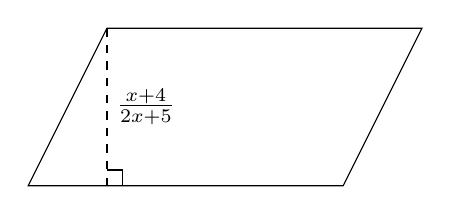
\begin{tikzpicture}
\draw (0,0) -- (4,0) -- (5,2) -- (1,2) -- cycle;
\draw[dashed] (1,2) -- (1,0);
\node[right] at (1,1) {$\frac{x+4}{2x+5}$};
\draw (1,0.2) -- (1.2,0.2) -- (1.2,0);
\end{tikzpicture} \\
\answer{The length of the base of the parallelogram is $\frac{3}{5}$ units.}
\end{practice}

\begin{practice}{38}{1}
Which of the following rational expressions simplify to $\frac{y}{y+3}$? Select all that apply. \\
$\square \; \frac{(2y^2+y)(y+3)}{(4y+2)(y+3)^2}$ \\
$\square \; \frac{3y^2+y}{3y^2+10y+3}$ \\
$\square \; \frac{2y^3+3y^2+y}{(2y+1)(y^2+4y+3)}$ \\
$\square \; \frac{y^2+2y}{y^2+4y+3}$ \\
$\square \; \frac{\frac{1}{y}}{y+3}$ \\
\answer{The second and third choices ($\frac{3y^2+y}{3y^2+10y+3}$ and $\frac{2y^3+3y^2+y}{(2y+1)(y^2+4y+3)}$) apply.}
\end{practice}

\begin{practice}{39}{1}
\textbf{SAT/ACT} For what value of $x$ is $\frac{2x^2+8x}{(x+4)(x^2-9)}$ undefined? \\
A. $-8$ \\
B. $-3$ \\
C. $0$ \\
D. $4$ \\
E. $9$ \\
\answer{B}
\end{practice}

\begin{practice}{40}{2}
\textbf{Performance Task} The approximate annual interest rate $r$ of a monthly installment loan is given by the formula:
$r = \frac{24(nm - p)}{n\left(p + \frac{nm}{12}\right)}$,
where $n$ is the total number of payments, $m$ is the monthly payment, and $p$ is the amount financed. \\
\textbf{Part A} Find the approximate annual interest rate (to the nearest percent) for a four-year signature loan of \$20,000 that has monthly payments of \$500. \\
\answer{9\%} \\
\textbf{Part B} Find the approximate annual interest rate (to the nearest tenth percent) for a five-year auto loan of \$40,000 that has monthly payments of \$750. \\
\answer{4.6\%}
\end{practice}

\end{document}